\chapter{Literature Review}
\label{ch:chapter_two}%
% The \label{...}% enables to remove the small indentation that is generated, always leave the % symbol.


\section{Introduction}
\label{sec:Introduction}

Self-balancing two-wheeled vehicles, inspired by the Segway, have garnered significant attention for their unique balancing mechanisms and versatile applications. This thesis focuses on a specific implementation of such technology: a self-balancing two-wheeled inverted pendulum (TWIP) designed to function as a smart trolley. This smart trolley is planned to autonomously follow its owner, providing assistance with tasks such as shopping or delivery.

The control systems of these smart trolleys are critical to ensure their stability, maneuverability, and ability to effectively follow a human operator. This chapter provides a comprehensive review of the existing literature on control methodologies for self-balancing TWIP, emphasizing applications similar to our smart trolley.

The control side of such vehicles involves addressing several complex challenges, including maintaining balance, navigating varied terrains, and accurately following a user. Researchers have explored a variety of control strategies to tackle these challenges, ranging from classical control methods to advanced algorithms based on artificial intelligence and machine learning.

Based on existing research, this chapter ends with a first description of our contribution: modeling the smart trolley as a floating-base system and applying \textit{Task Space Inverse dynamic} (TSID) control, a technique commonly used in humanoid robotics.
This approach aims to enhance stability, safeness, and responsiveness, tailored specifically for autonomous smart trolleys.

Before exploring the existing control approaches, an initial overview of Segway-like vehicles is provided.

\section{Overview of Segway-Like Vehicles}
\label{sec:Overview of Segway-Like Vehicles}

Segway vehicles, or self-balancing two-wheeled personal transporters, were invented by the American engineer Dean Kamen, in the early 2000s. Kamen introduced the Segway PT (Personal Transporter) in 2001 with the vision of revolutionizing short-distance travel and enhancing mobility in urban environments. The Segway's unique self-balancing technology and electric propulsion system set it apart from traditional modes of transport.

\begin{figure}
    \centering
    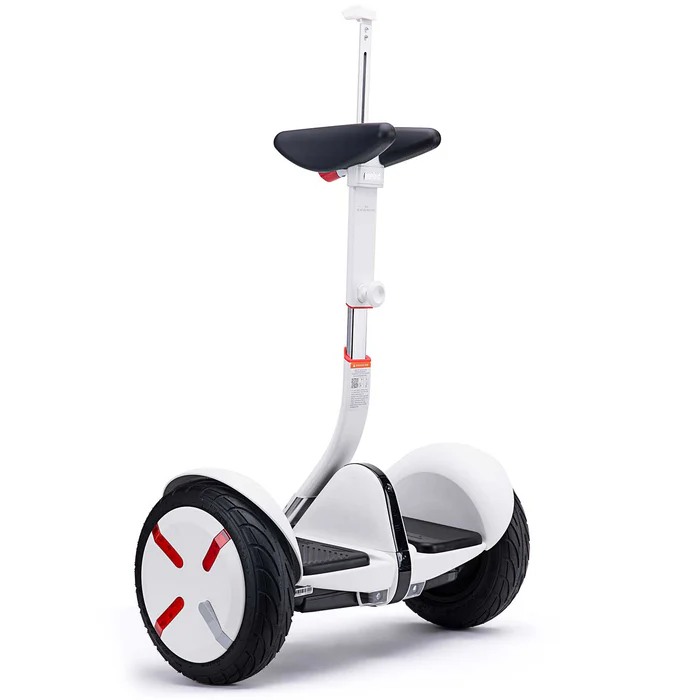
\includegraphics[width=0.5\linewidth]{Segway.png}
    \caption{Classical segway vehicle.}
    \label{fig:segway}
\end{figure}

The Segway PT's design allows for smooth and intuitive movement, controlled by shifting body weight, making it accessible to a wide range of users.

Segway vehicles have found diverse applications since their introduction. They are commonly used in urban commuting, offering a practical solution for "last-mile" travel, where public transportation might fall short. Additionally, they have become a popular choice for guided tours in cities, parks, and historical sites, providing a novel and enjoyable way to explore large areas.

In addition, Segways have been adapted for various specialized uses. In warehouses and large industrial facilities, they facilitate efficient movement of workers, enhancing productivity. Their potential extends to recreational activities and personal mobility for individuals with mobility challenges, contributing to an improvement in the quality of life.

The field of application of such vehicles is mainly circumscribed to the human-controlled side, in the sense that the rider has to change the speed, maneuver the robot with the handlebar to follow a desired trajectory, and stop.

Only in recent years the research is exploring the field of motion planning for Segway robots in order to achieve an autonomous trajectory tracking, while guaranteeing self-balancing, with the final aim of autonomous navigation.
The application area of such vehicles is wide: it can range from personal transportation of people with locomotion or visual impairments, different delivery purposes, or just simple object carrying to simplify peoples' everyday life.

The main objective of this literature review is to examine the different control techniques applied to self-balancing two-wheeled vehicles, their underlying principles, and their effectiveness.

\section{Fundamental Dynamical Properties of Segway-Like Vehicles}
\label{sec:Fundamental Dynamical Properties of Segway-Like Vehicles}

Before entering in the details of the various control methodologies, it is essential to highlight some key aspects that make the development of control algorithms for these systems particularly challenging. Understanding these fundamental points helps to explain why the study and refinement of control strategies for Segway-like vehicles have been a significant focus of research over the past 20 years an it is still ongoing.
First of all, these mechanical systems belong to the class of \textbf{Non-Linear systems}, where the laws governing the time evolution of state variables depend on their values in a manner that deviates from proportionality \cite{Khalil-2002}.
For these systems the superposition principle doesn't hold and stability analisys is much more complicated with respect to linear cases.
Moreover there are some \textit{essentially non linear phenomena} that can take place only in the presence of non linearity, among which we can mention the presence of \textbf{multiple isolated equilibria} and \textbf{limit cycles}.
Because of the powerful known tools for linear systems, the first step in analyzing a nonlinear system is usually to linearize it, but it means accepting all the limitations and approximations that derive from it.
Among this class of mechanical system, segways belongs to the subclass of underactuated mechanical systems, meaning that the number of actuators is less than the number of the system's degrees of freedom.
The study of underactuated systems has been extensively researched over the past three decades \cite{underactuated, spong2020robot}. This subclass includes significant mechanical structures such as the acrobot and the cartpole. More crucially, it encompasses all floating-base multibody systems, as discussed earlier in \cref{subsec: Floating-Base generalized coordinates}.
It is well-established \cite{Spong-underactuated} that fully actuated robots can be linearized via nonlinear feedback. Regarding underactuated robots, it is understood that the dynamic of the actuated (or active) degrees of freedom can be linearized using nonlinear feedback, while the residual dynamic following this partial linearization remain nonlinear and represent internal dynamic, requiring careful management.
The last important feature to be addressed, is something hidden inside the dynamic of the system and related to the specific configuration of the TWIP, with the body in its upright stable position:
After the linearization about that specific equilibrium, the linearized system is a \textbf{non-minimum phase system}, since the Input-Output \textit{transfer function} possesses a zero with positive real part \cite{Slotine1991AppliedNC, Hoagg-Nonminimum-phase-zeros}.
From the control perspective, performance can be limited because achieving high performance often requires high controller gains. However, high gains can lead to instability, as closed-loop poles tend to move towards open-loop zeros when the loop is closed.
The general outcome of this discussion is that controllers that imply dynamic cancellation may cancel that unstable zero with an unstable pole causing two main issues:

\begin{itemize}
    \item Any arbitrarily small discrepancy between the positive zero and the corresponding positive pole results in instability.  
    \item Even when the cancellation is perfect, an unstable controller pole cannot be used to cancel a nonminimum-phase plant zero because than that pole in closed loop is "\textit{no more a pole}", but still an eigenvalue, hiding an unstable dynamic that we are no more able to see and control \cite{Zhou1997EssentialsOR}.
\end{itemize}

All the mentioned features make TWIPs an interesting challenge from control-design perspective

\section{Review on existing control methodologies}
\label{sec:Review on existing control methodologies}

Considering all the challenges discussed thus far, this section provides an overview of the controllers that have been developed, highlighting their limitations and presenting our contributions.

We tried to categorize similar controllers, and briefly examine one by one each category.
\\

\begin{itemize}
    \item \textbf{Linear Classical and Optimal Control Methods.}  
    \item \textbf{Non-Linear Control Methods.} 
    \item \textbf{Intelligent Control Methods.} 
\end{itemize}


\subsection{Linear Classical and Optimal Control Methods}
\label{subsec:Linear Classical and Control Methods}

A common approach when dealing with a non linear system is trying to locally linearize it and exploit the various controllers known for linear systems.
Starting with model-free controllers, in \cite{Hyung-Jik-Lee} they estimated the pitch angle trough a sensor-fusion technique and then developed a single level control loop made up by a PD controller for the pendulum pitch angle and a PID controller for the position control of the system.
In \cite{Purohit2021KinematicCO} authors implemented a similar control strategy, with the difference that in this case the controller gains have been derived through a model-based approach (pole placement), starting from the linearization of the system about its unstable upright equilibrium position.
A similar approach has been followed in \cite{Johnson-et-al, Babazadeh-et-al}, comparing the results obtained with a simple PID controller, and Optimal Control theory (LQR).
The most important difference between them is that the the Optimal Control approach is based on a \textit{model} of the system, usually obtained from its equations of motion.
Then the controller gains are obtained through the minimization of a given \textit{cost functional} depending on the state-input trajectory \cite{Liberzon-calculus-of-var}.
Authors also show that LQR overperforms the simple PID, and the results improved if a precompensator is added.
The advantages of these kind of linear controllers are that they are easy to be implemented, and can work fine with a system like a TWIP because most of the time the body of the pendulum remains vertical or anyway in the neighborhood of that equilibrium, so the linearized systems behavior approximates very good the non linear one.
The drawback is that if we want to achieve higher performances in terms of accelerations and fast response, due to the system dynamic, the pitch angle has to increase accordingly, bringing the system away from its equilibrium position, making the linearized system no more reliable.
A further discussion about Optimal Control Theory is done in next chapters to highlight the main common aspects and differences with our approach.

\subsection{Non Linear Control Methods}
\label{subsec:Non Linear Control Methods}

 This review highlights the most commonly adopted non-linear control strategies for Segway control, although other approaches can be found: 

\begin{itemize}
    \item \textbf{Feedback Linearization Control (FLC)}: This is a non-linear control technique that transforms a non-linear system into an equivalent linear system through a change of variables and a nonlinear feedback control law. Essentially, it cancels out the system's non-linear dynamic, allowing linear control techniques to be applied across the entire state-space.
    It is important to note, as mentioned in the previous section, that underactuated systems cannot be fully feedback linearized \cite{Henson-et-al, Sastry1999}. Only a portion of these systems can be linearized, while the so-called internal dynamic remain non-linear. 
    This approach is known as \textbf{Partial Feedback Linearization (PFL)}. In PFL, the coordinate transformation can be complex, and ensuring the stability of the system is not always achievable.
    \\
    In \cite{Acosta-et-al} they apply PFL to the simple case of the \textit{cartpole}, while in \cite{Pathak-et-al} they do the same for the TWIP.
    In both cases they start from the dynamical model of the system obtained throguh the Newton-Euler equations, find an appropriate non-linear change of variables and derive the non-linear feedback control law; the internal dynamic stability is then guaranteed defining a proper Lyapunov Function respecting the Lyapunov second theorem for stability.
    
    \item \textbf{Model Predictive Control (MPC)} \cite{Liuping-MPC}: Model Predictive control is a control strategies involving the use of a model of the plant; the core of this algorithm is the following: knowing the new state measurement at each time step, this sample is used to solve an Optimal Control Problem with a \textit{finite time horizon}. Then only the first element of the control input trajectory is applied and this scheme is repeated at each time step.
    It is one of the most used control strategy in industry being able to handle both linear and non-linear systems with multiple control variables, and to its prediction functionality. 
    \\
    In \cite{Prabhakar-et-al} authors use MPC for the stabilization of a TWIP, developing the control algorithm in MATLAB, and testing it on a real robot; also in this case they compared the results with the one obtained through a simple PID and GA tuned PID, showing that the stabilization obtained through MPC is faster.
\end{itemize}


\subsection{Intelligent Control Methods}
\label{subsec:Intelligent Control Methods}

Intelligent controllers are advanced control systems that utilize artificial intelligence techniques, such as fuzzy logic, neural networks, and adaptive algorithms, to manage complex, nonlinear, and dynamic systems more effectively than traditional control methods. They can learn, adapt, and make decisions based on input data and environmental changes.
In many situations it is not possible to obtain precise mathematical model of the system due to its complexity and intelligent controllers can solve this problem.

\textbf{Fuzzy Logic Control}

FLC can be a MIMO system and it is based on three main steps:

\begin{itemize}
    \item Fuzzification: the process of transforming physical values to fuzzy values with the help of membership functions ranging from 0 to 1.
    \item Fuzzy Interference Process: it combines membership functions with some specific fuzzy rules, to derive the fuzzy output. 
    \item Defuzzification: it is the process that converts aggregated fuzzy sets into classical output values.
\end{itemize}
In \cite{Ahmad-et-al}, a fuzzy parallel distributed compensation (PDC) controller is introduced and implemented. They adopted the Takagi–Sugeno (TS) fuzzy model to obtain the state feedback gains required by solving the linear matrix inequalities (LMI). The results show that if strictly feasible solutions are found for the controller gains, then the fuzzy PDC controller performs better than the PID controller.
In some other approaches FL can be combined with conventional controllers obtaining a mixed control strategy: in \cite{Goher-et-al, Wu-et-al} they work on an hybrid Fuzzy/PID controller, based on the state-space model of the system, focusing on a robusteness anlisys against the model parameters.

\textbf{Neural Networks Control}

Neural networks and AI control for Segway and other two-wheeled inverted pendulum (TWIP) systems offer adaptive and robust performance by learning from data. These methods can handle complex, nonlinear dynamic and improve over time. However, they require substantial training data, computational resources, and can be challenging to interpret and debug compared to traditional control methods.
In \cite{Bature2016INTELLIGENTCF}, they explore the use of three different intelligent control methods: Fuzzy Logic Control (FLC), Neural Network Inverse Model Control (NN), and Adaptive Neuro-Fuzzy Inference System (ANFIS), for maintaining the balance and desired velocity of a two-wheeled inverted pendulum (TWIP) robot, showing that all three controllers performed well in simulations for both the tasks.
In \cite{Ahmed-et-al} it is shown an alternative control method using neural networks to replace PID controllers for controlling the cart position and handlebar angle of Segways, showing that neural network controllers are effective replacements for classical controllers, offering improved stability and performance.

Other relevant studies have been done wit intelligent controllers, all showing good results in terms of increasing performances, but with the cost of additional complexity, including dependency on the designer's expertise for fuzzy logic controllers, high energy consumption in neural network models, and the need for substantial training data.
Moreover, these methods often require significant computational resources and may not generalize well from simulations to real-world applications, posing challenges in practical deployment and tuning.

\section{Identified Challenges and Our Solutions}
\label{sec:Identified Challenges and Our Solutions}

The control of segway vehicles have been deeply explored, starting from simpler configurations like the cartpole, ending up with the final one.
Each of the previously mentioned works has its own advantages and drawbacks, and can be applied depending on the required performance.
The main outcomes regarding the actual state-of-art are the following:

Linear controllers have been the first one adopted, since they don't require the model of the system in the most of the cases, but the performances are limited by the linear approximation made for this strongly non-liner system.

Non linear model-based controllers instead have better performances with respect to the previously mentioned class, both in terms better tracking and faster stabilization. The main drawback is that they rely on the model of the system based on a reduced Lagrangian approach: starting from the conventional derivation of \textbf{EoM} the strong assumption that have been made is the no-slip constraint linking the wheels' axle center to the wheel's rotation.
This means that only one of the two variables is controlled, and if slip occurs, the controller can't do anything to correct it.

Intelligent controllers for Segway vehicles, depending on the application may not require a system model, and in general are able to achieve very good performances, with the cost of high energy consumption and significant computational resources.

For these reasons, the main contribution of this work has been the implementation of a non-linear controller (\textbf{Task Space Inverse dynamic, TSID}) where the no-slip condition is imposed as a constraint within an optimization problem.
Moreover the kinematic and dynamic model of the system have been written accordingly with the floating-base multibody convention, showing how a controller that has been in general adopted for humanoid robots, can perform effectively also with wheeled robots.

The aim of the next chapters will be that of providing a detailed description of Task Space Inverse dynamic, and how the conventional structure of the controller can be adapted to our case, in order to achieve good performance in terms of settling time and robustness with respect to model uncertainties.

\clearpage
\blankpage